%% LaTeX-Beamer template for KIT design
%% by Erik Burger, Christian Hammer
%% title picture by Klaus Krogmann
%%
%% version 2.0
%%
%% mostly compatible to KIT corporate design v2.0
%% http://intranet.kit.edu/gestaltungsrichtlinien.php
%%
%% Problems, bugs and comments to
%% burger@kit.edu

\documentclass[18pt]{beamer}
\usetheme{kit}

\titleimage{titleImage}
\titlelogo{logos}

% the presentation starts here

\title[MDP Pfadplanung]{Markov-Entscheidungsprozesse für die Roboterpfadplanung}
\subtitle{Entscheidungsprobleme unter Unsicherheit} %TODO nötig?
\author{Matthias Holoch}

\institute{Proseminar Anthropomatik: Von der Theorie zur Anwendung}

\begin{document}

\selectlanguage{ngerman}

%title page
\begin{frame}
	\titlepage
\end{frame}

%table of contents %TODO remove it, maybe
\frame{
	\frametitle{Gliederung}
	\tableofcontents
}

\section{Einleitung}
\begin{frame}
	\frametitle{Wozu das Ganze?}
	\begin{itemize}
		\item Lösen von Entscheidungsproblemen 
		\begin{itemize}
			\item Einbezug von Unsicherheiten
		\end{itemize}
		\visible<2->{
		\item Medizinische Diagnose
		\begin{itemize}
			\item genauer Patientenzustand unbekannt
			\item Menge an Therapiemöglichkeiten
			\item Beobachtungen als Hinweis auf den Patientenzustand
			\item Abwägen von Kosten
		\end{itemize}
		}
		\visible<3->{
		\item Roboterpfadplanung
		}
	\end{itemize}
\end{frame}

\section{Planung unter Unsicherheit}
\begin{frame}
	\frametitle{Planung unter Unsicherheit}	
	\visible<2,3>{
		\only<2>{
			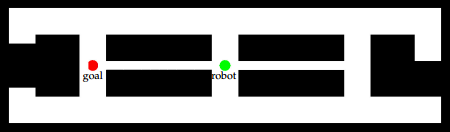
\includegraphics[scale=0.7]{images/autnmRobot_basicSituation.png}
		}
		\only<3>{
			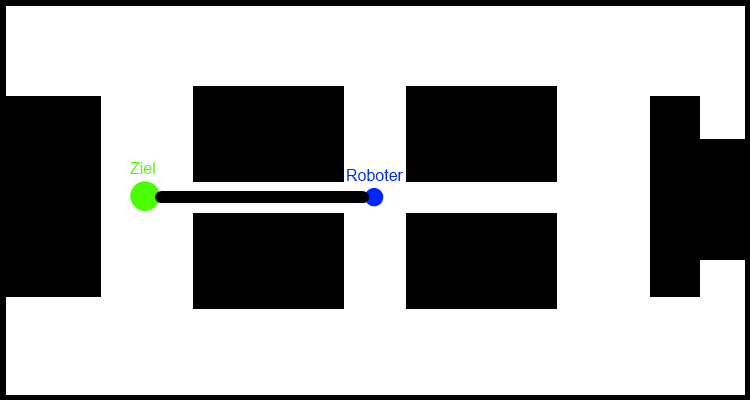
\includegraphics[scale=0.7]{images/autnmRobot_directPath.png}
		}
	}
	\begin{block}{Klassische Pfadplanung}
		Annahmen:
		\begin{enumerate}
			\item Genauer Zustand erkennbar
			\item Aktionsausführung fehlerfrei
		\end{enumerate}
		\only<4->{
		Probleme:
		\begin{itemize}
			\item the cake...
			\item it's a lie!
		\end{itemize}
		}
	\end{block}
\end{frame}

\section{MDP}

\section{Strategien}
\subsection{Optimale Strategie}
\subsection{Algorithmus}

\begin{frame}{~}
	\begin{center}
		\huge{DANKE FÜR DIE AUFMERKSAMKEIT!}
	\end{center}
\end{frame}

\end{document}
